On considère le cube $ABCDEFGH$.

On note $I$ le milieu du segment $[EH]$ et on considère le triangle $CFI$.

L'espace est muni du repère orthonormé $\left(A;\vect{AB},\vect{AD},\vect{AE}\right)$ et on admet que le point $I$ a pour coordonnées $\left(0;dfrac12;1\right)$ dans ce repère.

\begin{center}
	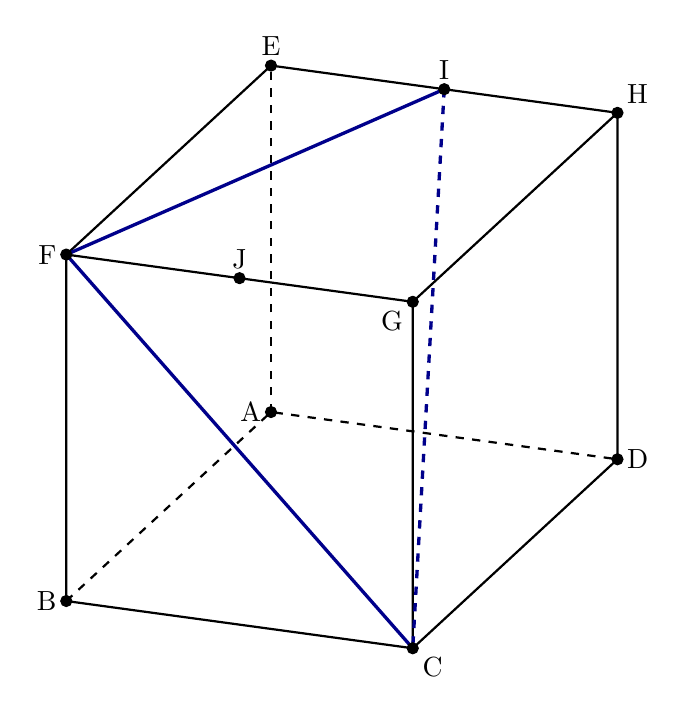
\begin{tikzpicture}[line join=bevel]
		\draw[thick] (0.2,0.8)--(4.6,0.2)--(4.6,4.6)--(0.2,5.2)--cycle;%BCGF
		\draw[thick] (4.6,0.2)--(7.2,2.6)--(7.2,7)--(4.6,4.6);%CDHG
		\draw[thick] (7.2,7)--(2.8,7.6)--(0.2,5.2);%HEF
		\draw[thick,dashed] (0.2,0.8)--(2.8,3.2)--(7.2,2.6);%BAD
		\draw[thick,dashed] (2.8,3.2)--(2.8,7.6);%AE
		\draw[DarkBlue,very thick] (5,7.3)--(0.2,5.2)--(4.6,0.2);%I-F-C
		\draw[DarkBlue,very thick,dashed] (5,7.3)--(4.6,0.2);%IC
		\foreach \Point/\Nom/\Pos in {(2.8,3.2)/A/left,(0.2,0.8)/B/left,(4.6,0.2)/C/below right,(7.2,2.6)/D/right,(2.8,7.6)/E/above,(0.2,5.2)/F/left,(4.6,4.6)/G/below left,(7.2,7)/H/above right,(5,7.3)/I/above,(2.4,4.9)/J/above}
		\filldraw \Point circle[radius=2pt] node[\Pos] {\Nom} ;
	\end{tikzpicture}
\end{center}

\begin{enumerate}
	\item 
	\begin{enumerate}
		\item Donner sans justifier les coordonnées des points $C$, $F$ et $G$.
		\item Démontrer que le vecteur $\vect{n}\begin{pmatrix}1\\2\\2\end{pmatrix}$ est normal au plan $(CFI)$.
		\item Vérifier qu'une équation cartésienne du plan $(CFI)$ est : $x + 2y + 2z - 3 = 0$.
	\end{enumerate}	
	\item  On note $d$ la droite passant par $G$ et orthogonale au plan $(CFI)$.
	\begin{enumerate}
		\item Déterminer une représentation paramétrique de la droite $d$.
		\item Démontrer que le point $K\left(\dfrac79~;~\dfrac59~;~\dfrac59\right)$ est le projeté orthogonal du point $G$ sur le plan $(CFI)$.
		\item Déduire des questions précédentes que la distance du point $G$ au plan $(CFI)$ est égale à $\dfrac23$.
	\end{enumerate}
	\item On considère la pyramide $GCFI$.
	
	\emph{On rappelle que le volume $\mathcal{V}$ d'une pyramide est donné par la formule} \[\mathcal{V} = \frac13 \times b \times h,\]
	%
	\emph{où $b$ est l'aire d'une base et $h$ la hauteur associée à cette base}.
	\begin{enumerate}
		\item Démontrer que le volume de la pyramide $GCFI$ est égal à $\dfrac16$, exprimé en unité de volume.
		\item En déduire l'aire du triangle $CFI$, en unité d'aire.
	\end{enumerate}
\end{enumerate}